\chapter{Модель предлагаемого решения}
\label{chap:Modeling}

\section{Содержательная модель}
Система автоматического извлечения ключевых фраз из текста на
естественном языке выполняет выделение ключевых фраз из текста на
естественном языке с применением графематических шаблонов,
морфологического словаря (лексикона) и синтаксических правил.
Эти данные определены предварительно и хранятся в базе данных.

Текст обрабатывается графематическим анализатором, который
вырабатывает информацию о разделении текста на абзацы,
предложения и отдельные слова, необходимую для дальнейшей обработки.

Каждое слово, выделенное графематическим анализатором,
подвергается морфологическому анализу с целью построения
морфологической интерпретации (часть речи, форма, и\ т.\ д.),
определения основы слова и формирования леммы
(канонической формы лексемы).

На основе имеющейся графематической и морфологической
интерпретации текста, выполняется построение и наполнение
синтаксических групп, и выявление отношений между ними.

Ключевые фразы выделяются из именных групп, сформированных
синтаксическим анализатором при помощи статистического
метода C-value, поощряющего существование в тексте
ключевых фраз, не входящих в состав других, более длинных.

\section{Концептуальная модель}

\subsection{Общая модель}
Система автоматического извлечения ключевых фраз из текста
на естественном языке — программный комплекс, выполняющий \emph{функции}
статистического выделения ключевых фраз из текста на естественном
языке \emph{путём} графематического, морфологического, синтаксического
анализа текста \emph{на основе} определённых графематических шаблонов,
морфологических словарей, синтаксических правил и метрики C-value,
\emph{направленный на} автоматизацию процедуры извлечения ключевых фраз
\emph{с целью} формирования списка терминов по тексту.

\subsection{Базово--уровневая модель}
\textbf{Функции:} статистическое выделение ключевых фраз
из текста (определение списка терминов-кандидатов из именных
групп, подсчёт частоты появления в тексте каждого
термина--кандидата, вычисление значения терминологичности для
каждого термина--кандидата из списка).

\textbf{Пути реализации функций:}
построение графематической интерпретации входного текста
(разбиение текста на абзацы, предложения, подпредложения и отдельные
слова, определение языка слов); построение морфологической
интерпретации слов входного текста (выделение основ слов,
определение частей речи и соответствующих наборов граммем);
синтаксический разбор входного текста (построение синтаксических
групп на каждом морфологическом варианте каждого фрагмента
предложения, выявление связей между группами).

\textbf{Основы выполнения функций:} определённые
графематические шаблоны, морфологические словари и
синтаксические правила, метрика C-value.

\textbf{Направление реализации функций:} автоматизация
процедуры извлечения ключевых фраз из текста.

\textbf{Цель:} формирование списка терминов по тексту.

\subsection{Модификационная модель}
\textbf{Функции:} статистическое выделение ключевых фраз из текста
(определение списка терминов--кандидатов из именных групп, подсчёт
частоты появления в тексте каждого термина--кандидата,
нахождение терминов--кандидатов в составе других
терминов--кандидатов, подсчёт длины каждого термина-кандидата,
вычисление значения терминологичности для каждого термина--кандидата
из списка).

\textbf{Пути реализации функций:} построение графематической
интерпретации входного текста (разбиение текста на абзацы,
предложения, подпредложения и отдельные слова при помощи
детерминированного конечного автомата; определение языка каждого
слова при помощи регулярных выражений); построение морфологической
интерпретации слов входного текста (поиск оптимального разбиения
каждого слова на суффикс и основу слова, определение правил
внутренней флексии для словоформ, определение частей речи и
соответствующих наборов граммем по морфологическому словарю);
синтаксический разбор входного текста (построение синтаксических
групп на каждом морфологическом варианте каждого фрагмента предложения,
выявление связей между группами, идентификация вида каждой связи).

\textbf{Основы выполнения функций:} определённые
графематические шаблоны, морфологические словари и
синтаксические правила, метрика C-value.

\textbf{Направление реализации функций:} автоматизация
процедуры извлечения ключевых фраз из текста.

\textbf{Цель:} формирование списка списка терминов по тексту.

\section{Структурная модель}
Структурная модель предлагаемого решения приведена на
рисунке~\ref{fig:Solution-Rank0}. В структуру прототипа внесён
блок выделения ключевых фраз (выделено серым цветом),
рассматриваемый как готовое решение 1-го ранга, изображённое
на рисунке~\ref{fig:Solution-Rank1a}.

\begin{figure}[ht]
  \centering
  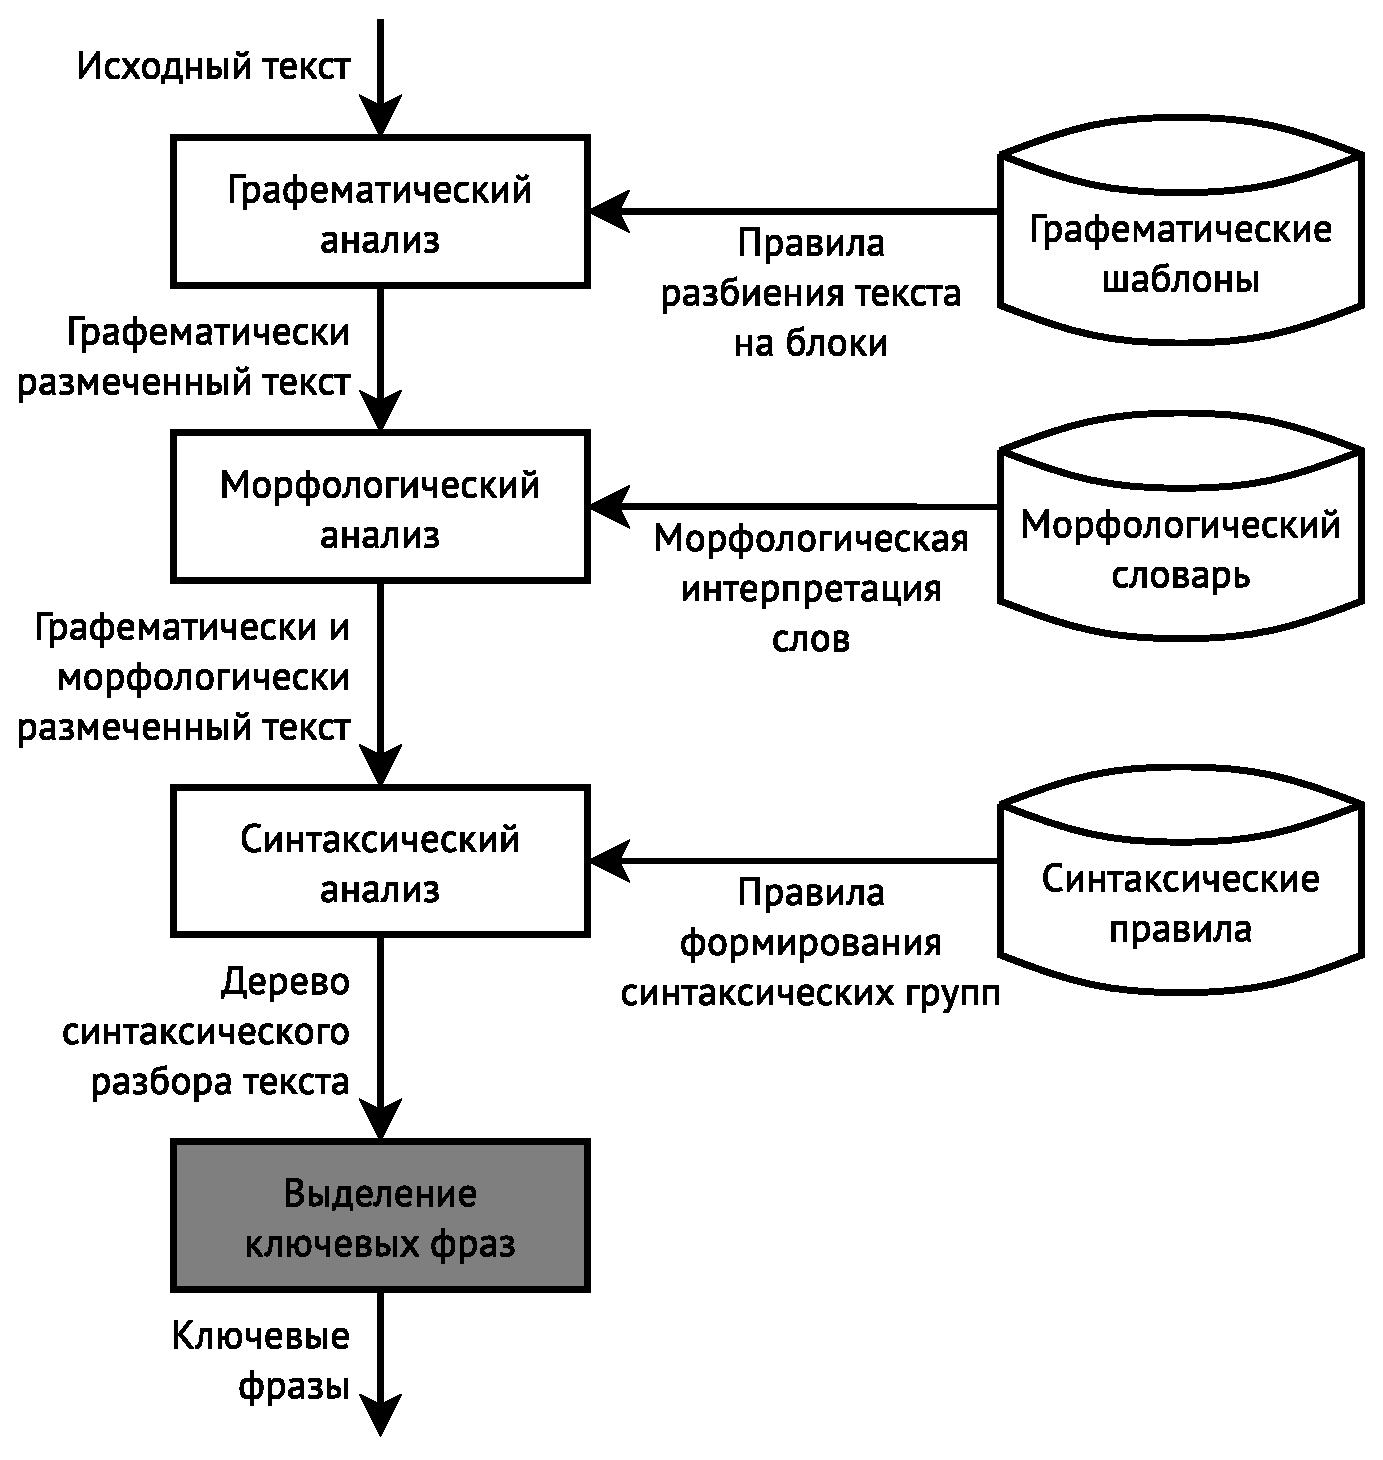
\includegraphics[scale=0.5]{Solution-Rank0.eps}
  \caption{Структурная модель предлагаемого решения}
  \label{fig:Solution-Rank0}
\end{figure}

\section{Функционально--структурная модель}
Функционально--структурная модель предлагаемой системы автоматического
извлечения ключевых фраз из текста на естественном языке построена при
помощи пакета Computer Associates ERwin Process Modeler 7.3 с
применением методологии проектирования SADT IDEF0 и приведена в
приложении~\ref{chap:FunctionalModels}.

На рисунке~\ref{fig:FunctionalModels:A-0} показано функционирование
системы с точки зрения разработчика (0-й уровень, контекстная
диаграмма). При последующей декомпозиции получается
функционально--структурная модель 1-го уровня (рисунок
\ref{fig:FunctionalModels:A0}).

Блок №4: «Выделить ключевые фразы» отсутствует в прототипе и был
внесён с целью преодоления его недостатков, обозначенных в
\ref{subsec:Critic}. Декомпозиция узла A4, соответствующего данному
блоку, представлена на рисунке~\ref{fig:FunctionalModels:A4}.

\section{Алгоритмическая модель}
Алгоритмическая модель предлагаемого решения приведена на
рисунке~\ref{fig:Solution-Algorithm-Rank0}. В алгоритм
функционирования прототипа внесено готовое решение 1-го ранга —
процедура выделения ключевых фраз (обозначено серым цветом),
алгоритм функционирования которой изображён на
рисунке~\ref{fig:Solution-Algorithm-Rank1a}.

\begin{figure}[!ht]
  \centering
  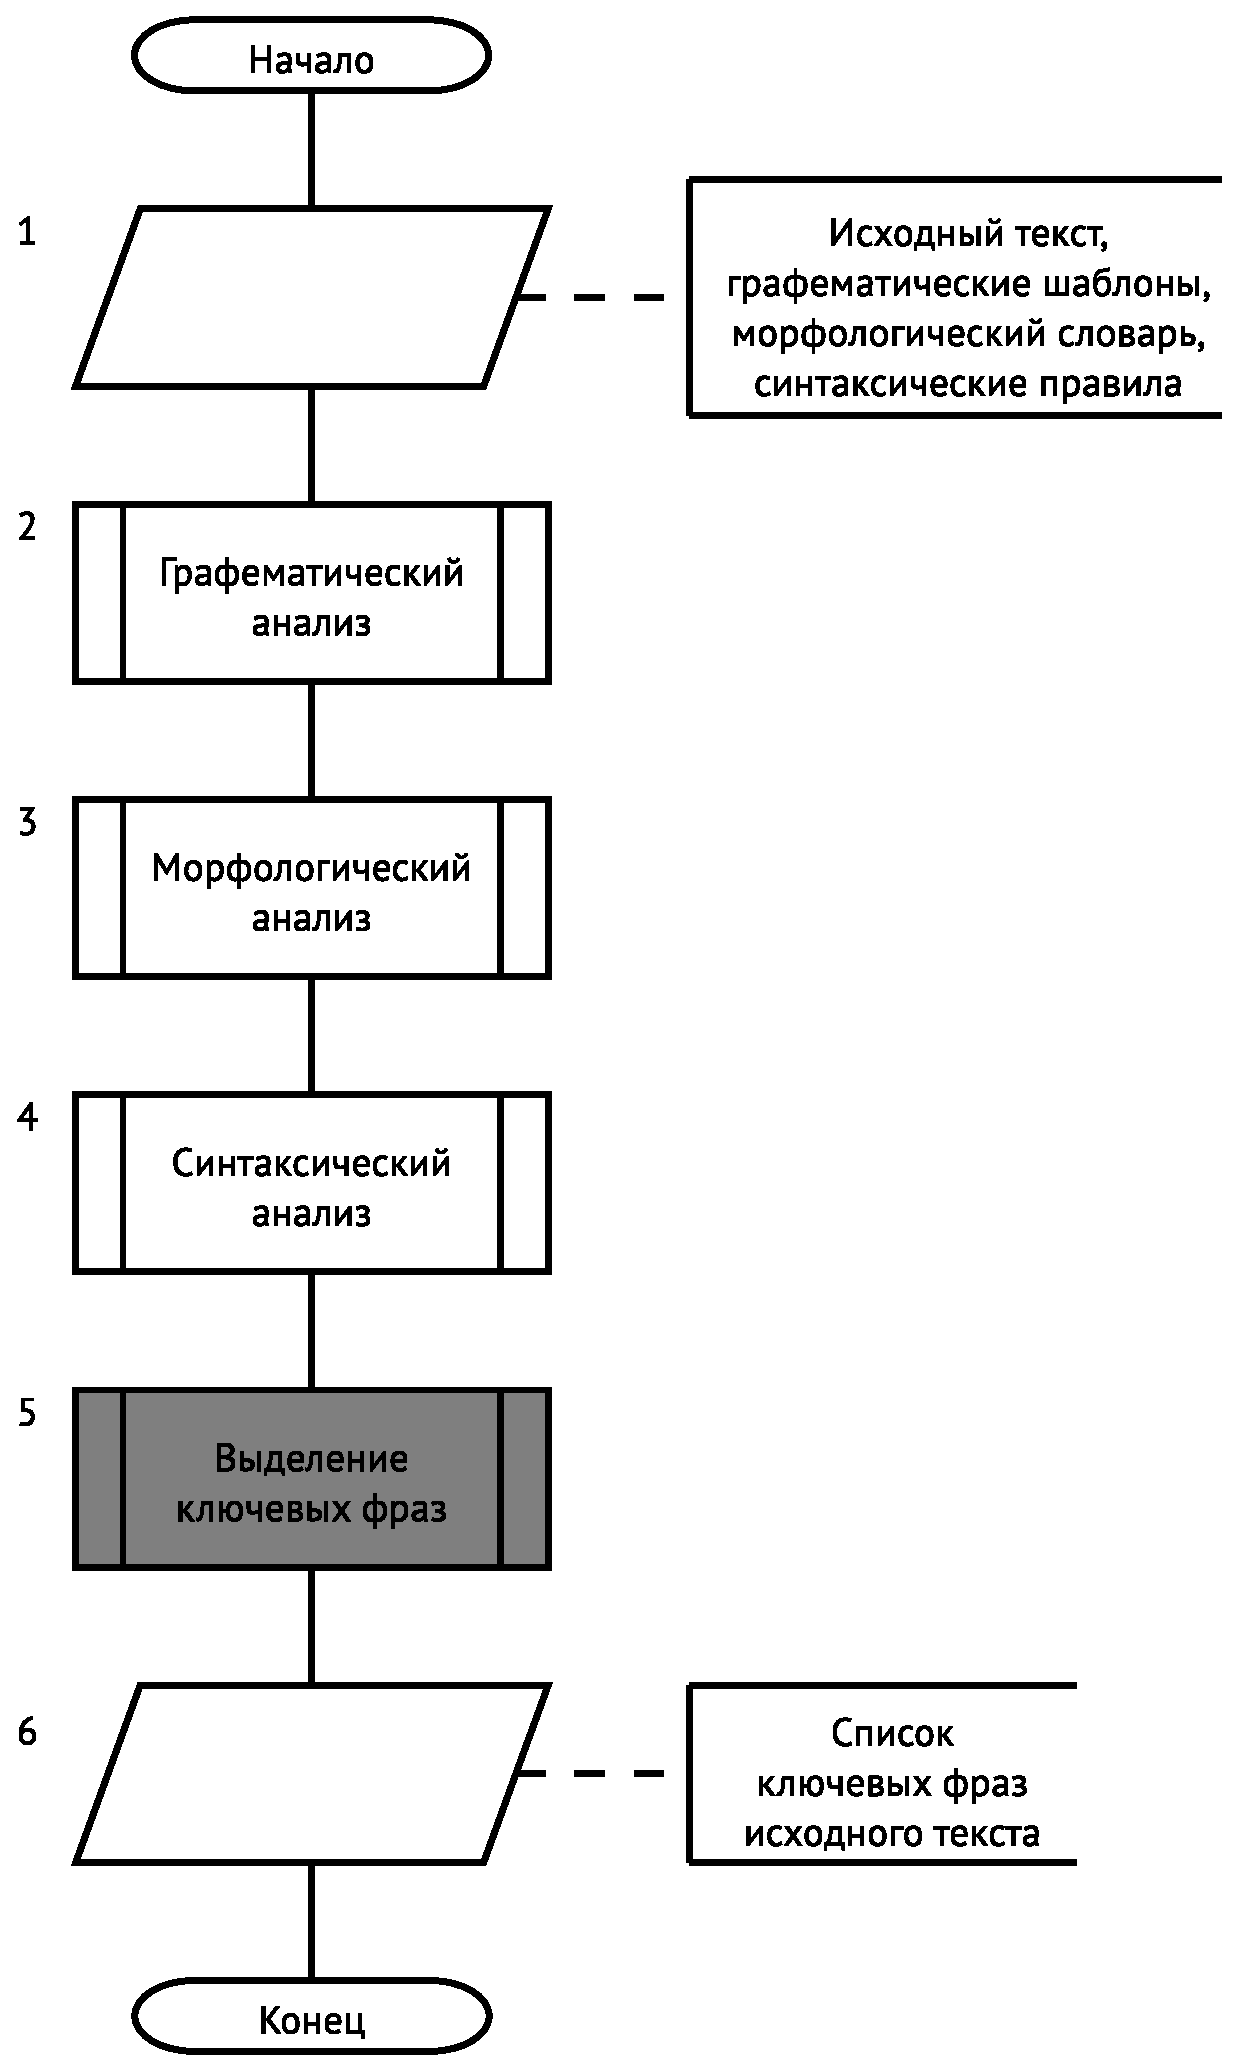
\includegraphics[scale=0.5]{Solution-Algorithm-Rank0.eps}
  \caption{Алгоритмическая модель предлагаемого решения}
  \label{fig:Solution-Algorithm-Rank0}
\end{figure}

\section{Результаты и выводы}
Были построены следующие модели предлагаемого решения:
\begin{itemize}
  \item содержательная модель;
  \item концептуальные модели: общая, базово--уровневая и
модификационная;
  \item структурная модель;
  \item функционально--структурная модель;
  \item алгоритмическая модель.
\end{itemize}

Разработанный пакет моделей системы автоматического извлечения
ключевых фраз из текста на естественном языке даёт представление
о принципах её функционирования, концептуальном устройстве,
а также структурном составе.

Созданный пакет моделей позволяет провести проектирование системы
автоматического извлечения ключевых фраз из текста на естественном
языке, устранив основные недостатки прототипа, обозначенные в
\ref{subsec:Critic}.
